\documentclass[10pt,twocolumn,preprint]{emulateapj}
\usepackage[english]{babel}
\usepackage{amsmath}

\newcommand{\bs}{\boldsymbol}
\newcommand{\diff}{{\mathrm d}}
\newcommand{\Cov}{\mathsf{C}}
\newcommand{\Fish}{\mathsf{F}}
\newcommand{\Cl}{\mathcal {C}}
\newcommand{\R}{\mathcal{R}}
\newcommand{\T}{\mathcal{T}}
\newcommand{\Msun}{M_\odot}


%\shortauthors{Author et al.} \shorttitle{New CubeP3M}
\begin{document}
\title{New $N$-body Algorithm}
\author{Authors}

\affil{Affiliations}

\email{email@email.email}

\begin{abstract}
We present a memory-lite $N$-body algorithm.
\end{abstract}

\keywords{}

\maketitle

\section{Introduction}
$N$-body simulations are important. Citation \cite{2000ApJ...534L..19P}.  Bold type use $\bs{v}=\vec{v}$.


\begin{figure} \centering
  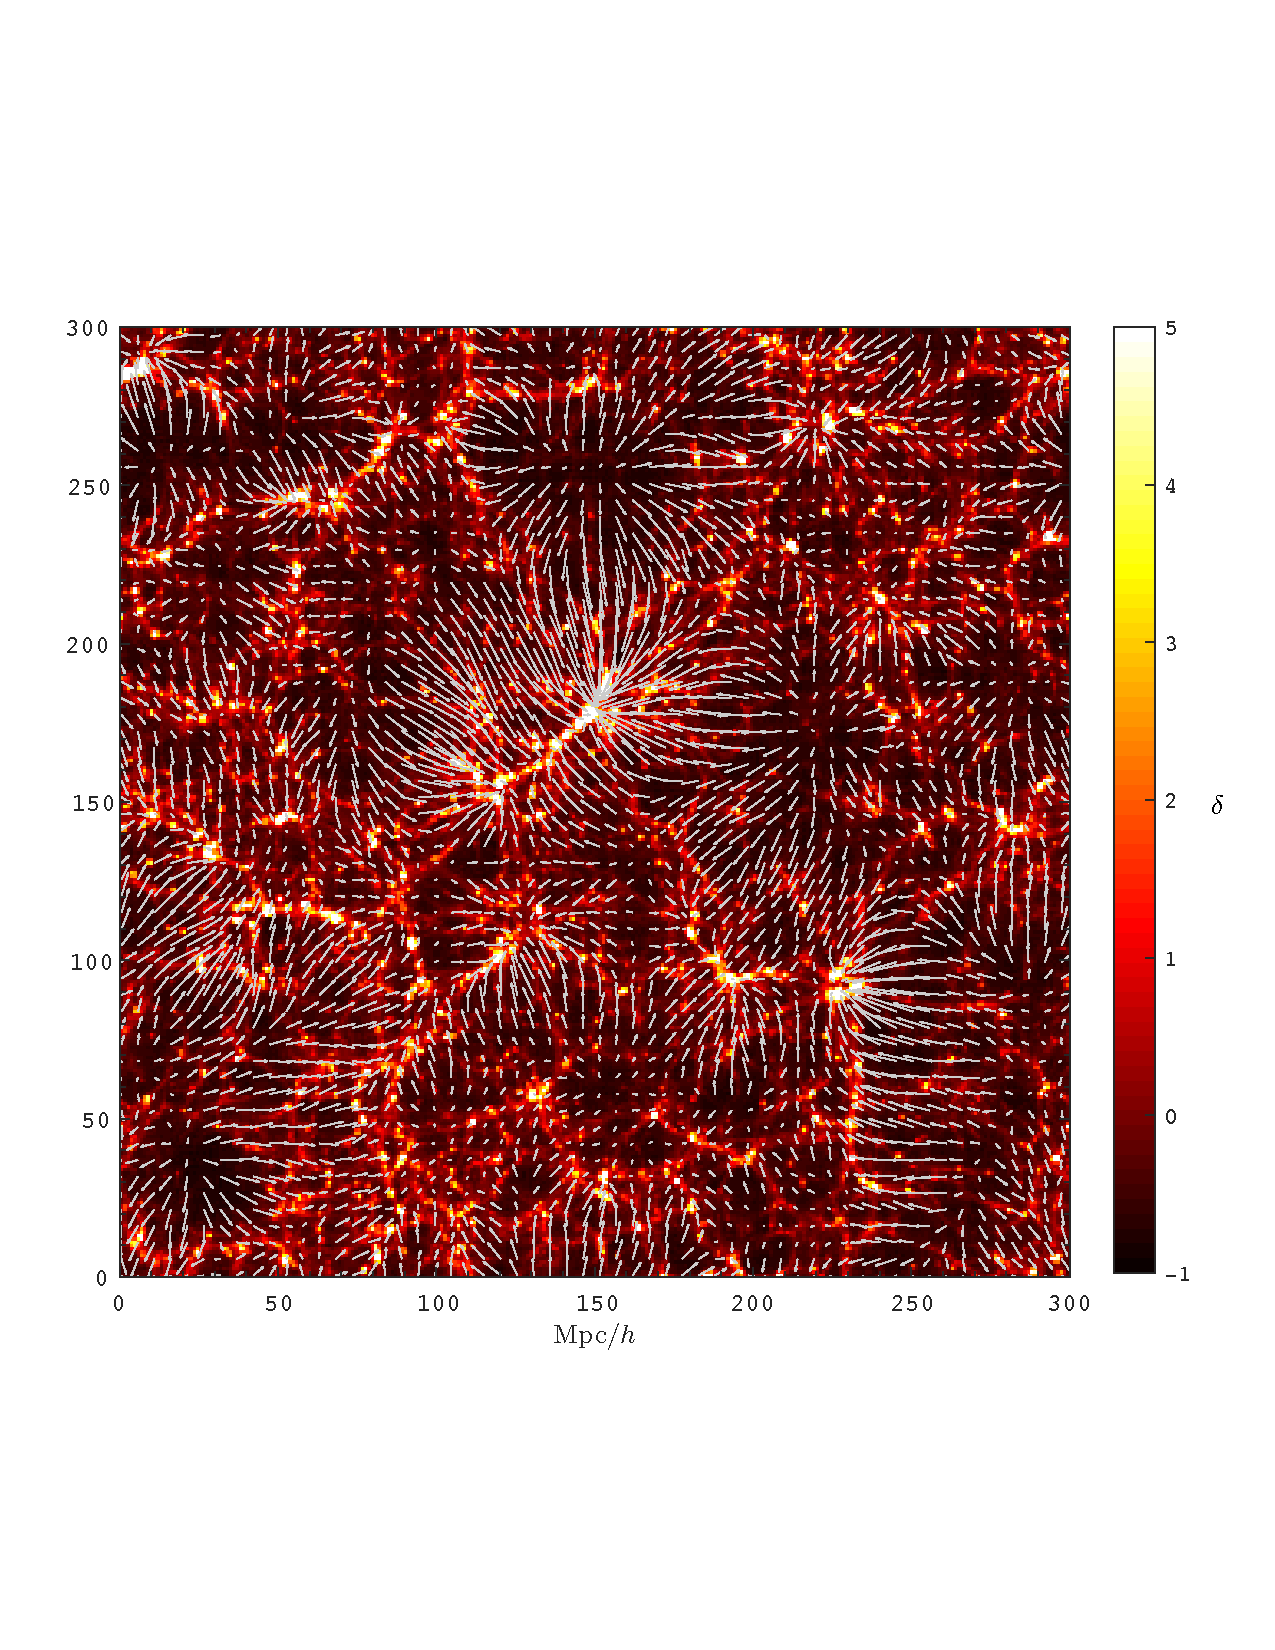
\includegraphics[width=1.0\linewidth]{fig1.pdf}
  \caption{Caption goes here.}
  \label{fig.1}
\end{figure}

\section{Conclusion}
We present a memory-lite $N$-body algorithm.

\acknowledgements
Thanks.

\bibliographystyle{hapj}
\bibliography{../haoran_ref}

\end{document}
